\message{ !name(article.tex)}%% Copernicus Publications Manuscript Preparation Template for LaTeX Submissions
%% ---------------------------------
%% This template should be used for copernicus.cls
%% The class file and some style files are bundled in the Copernicus Latex Package, which can be downloaded from the different journal webpages.
%% For further assistance please contact Copernicus Publications at: production@copernicus.org
%% https://publications.copernicus.org/for_authors/manuscript_preparation.html


%% Please use the following documentclass and journal abbreviations for discussion papers and final revised papers.

%% 2-column papers and discussion papers
\documentclass[npg,manuscript]{copernicus}


%% Journal abbreviations (please use the same for discussion papers and final revised papers)


% Advances in Geosciences (adgeo)
% Advances in Radio Science (ars)
% Advances in Science and Research (asr)
% Advances in Statistical Climatology, Meteorology and Oceanography (ascmo)
% Annales Geophysicae (angeo)
% Archives Animal Breeding (aab)
% ASTRA Proceedings (ap)
% Atmospheric Chemistry and Physics (acp)
% Atmospheric Measurement Techniques (amt)
% Biogeosciences (bg)
% Climate of the Past (cp)
% DEUQUA Special Publications (deuquasp)
% Drinking Water Engineering and Science (dwes)
% Earth Surface Dynamics (esurf)
% Earth System Dynamics (esd)
% Earth System Science Data (essd)
% E&G Quaternary Science Journal (egqsj)
% Fossil Record (fr)
% Geographica Helvetica (gh)
% Geoscientific Instrumentation, Methods and Data Systems (gi)
% Geoscientific Model Development (gmd)
% History of Geo- and Space Sciences (hgss)
% Hydrology and Earth System Sciences (hess)
% Journal of Micropalaeontology (jm)
% Journal of Sensors and Sensor Systems (jsss)
% Mechanical Sciences (ms)
% Natural Hazards and Earth System Sciences (nhess)
% Nonlinear Processes in Geophysics (npg)
% Ocean Science (os)
% Primate Biology (pb)
% Proceedings of the International Association of Hydrological Sciences (piahs)
% Scientific Drilling (sd)
% SOIL (soil)
% Solid Earth (se)
% The Cryosphere (tc)
% Web Ecology (we)
% Wind Energy Science (wes)


%% \usepackage commands included in the copernicus.cls:
%\usepackage[german, english]{babel}
%\usepackage{tabularx}
%\usepackage{cancel}
%\usepackage{multirow}
%\usepackage{supertabular}
%\usepackage{algorithmic}
%\usepackage{algorithm}
%\usepackage{amsthm}
%\usepackage{float}
%\usepackage{subfig}
%\usepackage{rotating}
\usepackage{easy-todo}
\usepackage{graphicx}
\newcommand{\yobs}{\mathbf{y}^o}
\DeclareMathOperator*{\argmin}{arg\,min \,}
\DeclareMathOperator*{\argmax}{arg\,max \,}
\newcommand{\Var}{\mathbb{V}\textrm{ar}}
\newcommand{\Ex}{\mathbb{E}}
\newcommand{\Prob}{\mathbb{P}}
\newcommand{\Cov}{\textsf{Cov}}
\newcommand{\tra}{\mathrm{tr}}
\newcommand{\kmean}{\mathbf{k}_{\mathrm{mean}}}
\newcommand{\checkap}{\check{\alpha}_p}
\newcommand{\checkkp}{\check{\mathbf{k}}_p}
\begin{document}

\message{ !name(article.tex) !offset(91) }
\section{Calibration: deterministic twin experiments}
\label{sec:deterministic}
% \subsection{Parameter calibration in a deterministic setting}


For the estimation of the ``best'' value of $\mathbf{k}$, we adopt a twin experiment framework:
an observation $\yobs$ is generated with a couple of values $\mathbf{k}^t$ and $\mathbf{u}^t$, supposed unknown (where ${(\cdot)}^t$ stands for ``truth''):
\begin{equation}
  \yobs = \mathcal{M}(\mathbf{k}^t, \mathbf{u}^t)
\end{equation}
In a data assimilation setting, this calibration consists in the minimisation of the cost function $J$ defined by
\begin{align}
  \label{eq:def_cost_fun}
  J(\mathbf{k}) & = \frac12\|\mathcal{M}(\mathbf{k},\mathbf{u}^b) - \yobs \|_{\mathbf{R}^{-1}}^2 + \mathop{\mathrm{regul}}(\mathbf{k})%\frac12\|\mathbf{k}-\mathbf{k}^b\|_{\mathbf{B}^{-1}}^2
\end{align}
where $\mathop{\mathrm{regul}}$ is a regularisation function taking possibly into account a background value $\mathbf{k}^b$. The matrix $\mathbf{R}$ is the covariance matrix of the observation error. Assuming a well-posed problem, the function $J$ reaches a minimum for $\hat{\mathbf{k}}$:
\begin{equation}
  \label{eq:khat_def}
  J(\hat{\mathbf{k}}) = \min_{\mathbf{k} \in \mathcal{K}} J(\mathbf{k})
\end{equation}
Minimising $J$ will indeed compensate the error introduced by the parametrisation $\mathbf{k}$, but will also compensate another misspecification: choosing $\mathbf{u}^b$ instead of $\mathbf{u}^t$ in the computer code.
In the end, the value $\hat{\mathbf{k}}$ obtained will be optimal for this configuration. However, if the operating conditions do change, there is no information on the performance of $\hat{\mathbf{k}}$ for this other setting.
In turn, this may lead to poor results when the calibrated model is used to perform predictions.
% \begin{figure}[t]
% 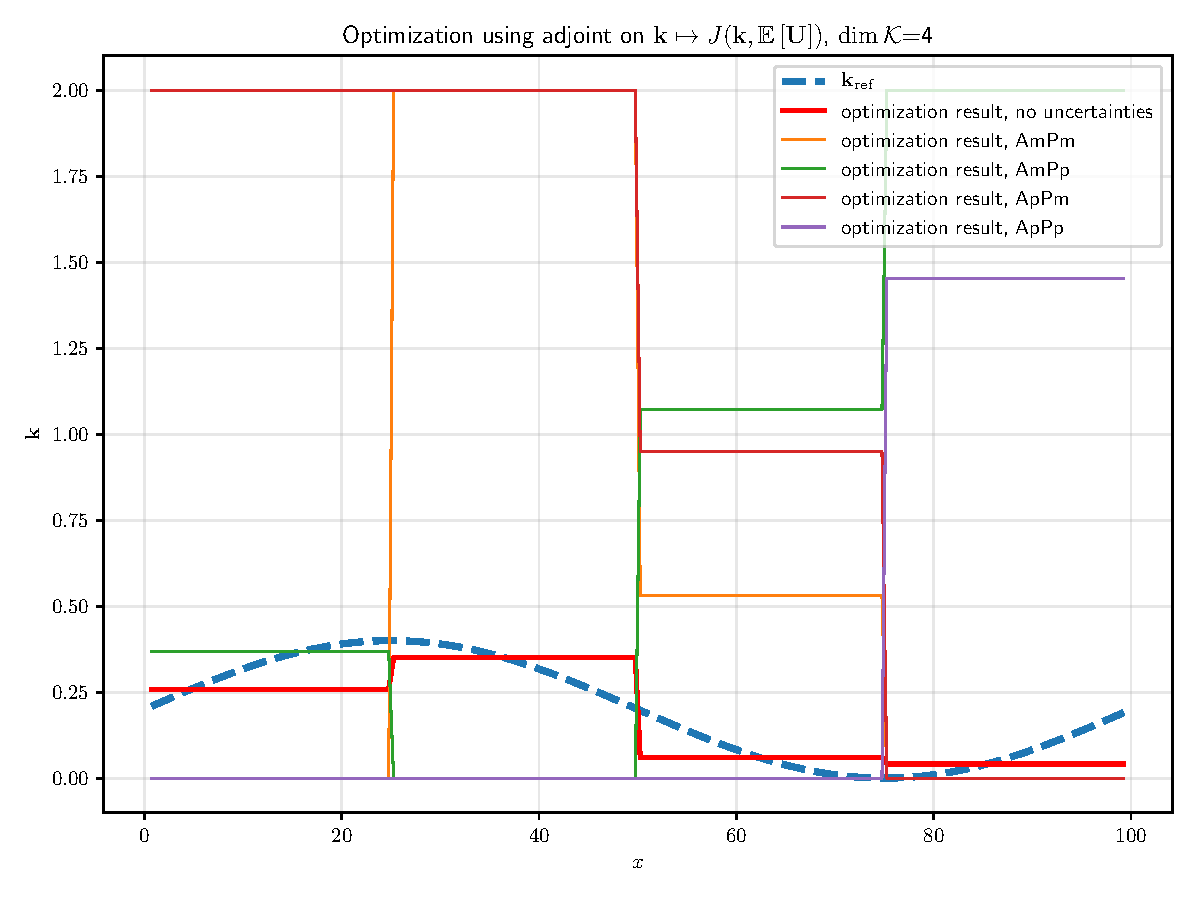
\includegraphics[width=8.3cm]{Figures/optimization_using_misspecified_uref_4d.pdf}
% \caption{TEXT}
% \end{figure}
% \begin{figure*}[t]
% 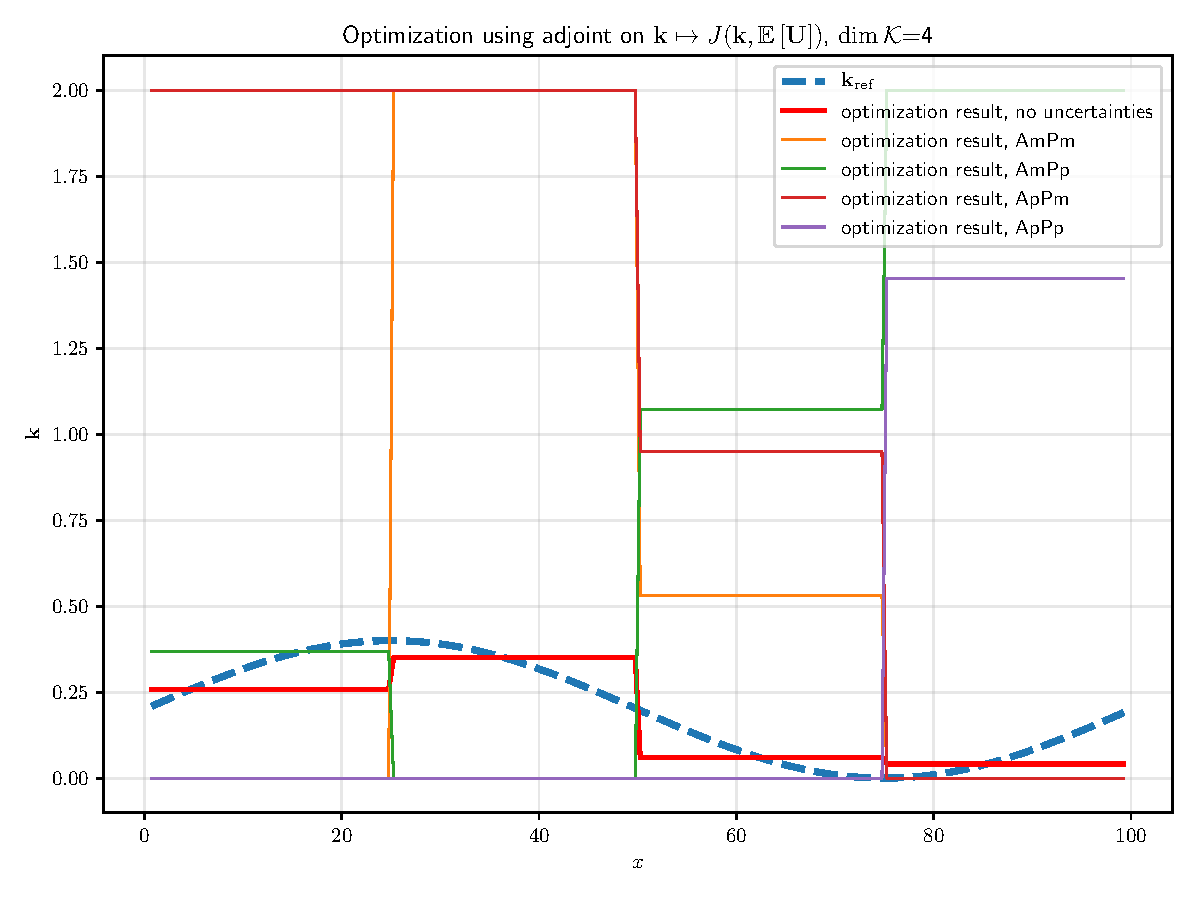
\includegraphics[width=12cm]{Figures/optimization_using_misspecified_uref_4d.pdf}
% \caption{TEXT}
% \end{figure*}


%----------------------------------------------------------------------------

\message{ !name(article.tex) !offset(812) }

\end{document}
